
\section{Experiments}
\subsection{실험 설정}
평가 데이터셋은 NetConfigQA~2.0의 4개 Lab으로 구성되며, 전체 QA 수는 9,462개이다. 모델은 4개 벤더에서 6개 LLM을 선정하였다.

\begin{table*}[!t]
  \caption{평가 모델 구성}
  \label{tab:model-setup}
  \centering
  \small
  \begin{tabular}{|L{2.6cm}|L{2.0cm}|L{3.0cm}|L{1.8cm}|C{1.5cm}|}
    \hline
    \textbf{모델}   & \textbf{벤더} & \textbf{파라미터}       & \textbf{양자화} & \textbf{Context} \\
    \hline
    GPT-4o-mini   & OpenAI      & -- (API)            & --           & 128K             \\
    \hline
    GPT-OSS-20B   & OpenAI      & 20B                 & MXFP4        & 131K             \\
    \hline
    Qwen3-Coder   & Alibaba     & 30B MoE / 3B active & Q4\_K\_M     & 256K             \\
    \hline
    Gemma-3-27B   & Google      & 27B                 & Q4\_K\_M     & 128K             \\
    \hline
    GLM-4.7-Flash & Zhipu       & 30B MoE / 3B active & Q4\_K\_M     & 198K             \\
    \hline
    Qwen3.5-27B   & Alibaba     & 27B                 & Q4\_K\_M     & 262K             \\
    \hline
  \end{tabular}
\end{table*}

모든 평가는 zero-shot 조건에서 수행하며, temperature는 0으로 고정하고 `num\_ctx`는 49,152로 설정하였다. 로컬 모델 서빙은 RTX 3090 (24GB) 환경의 Ollama를 사용하였다. 평가 지표는 TA-Acc와 Format Stability(Parse Success Rate)이다. 모델 간 성능 차이의 유의성은 Bootstrap 95\% 신뢰구간(10,000회 리샘플링)으로 검정한다. Single LLM 평가가 완료되면 Overall TA-Acc가 가장 높은 오픈소스 모델을 Pure MAS와 NetAlly의 공통 backbone으로 사용한다([TODO]: 모델명).

\subsection{Single LLM 기준선과 확장성}
LLM의 설정 파일 해석 능력을 평가하기 위해 6개 모델을 4개 Lab에 각각 적용하여 총 $6\times4=24$회 평가하였다.

\begin{table*}[!t]
  \caption{Single LLM 기준선: Overall TA-Acc (6개 모델 $\times$ 4개 Lab). 각 셀은 Micro / Macro 순이다.}
  \label{tab:single-llm-baseline}
  \centering
  \small
  \begin{tabular}{|L{2.8cm}|C{1.9cm}|C{1.9cm}|C{1.9cm}|C{1.9cm}|}
    \hline
    \textbf{모델}   & \textbf{Lab-A (10)} & \textbf{Lab-B (20)} & \textbf{Lab-C (30)} & \textbf{Lab-D (40)} \\
    \hline
    GPT-4o-mini   & [TODO]              & [TODO]              & [TODO]              & [TODO]              \\
    \hline
    GPT-OSS-20B   & [TODO]              & [TODO]              & [TODO]              & [TODO]              \\
    \hline
    Qwen3-Coder   & [TODO]              & [TODO]              & [TODO]              & [TODO]              \\
    \hline
    Gemma-3-27B   & [TODO]              & [TODO]              & [TODO]              & [TODO]              \\
    \hline
    GLM-4.7-Flash & [TODO]              & [TODO]              & [TODO]              & [TODO]              \\
    \hline
    Qwen3.5-27B   & [TODO]              & [TODO]              & [TODO]              & [TODO]              \\
    \hline
  \end{tabular}
\end{table*}

파이프라인 확장성은 QA/노드 비율로 함께 보고한다. 본 데이터셋에서는 Lab-A 126, Lab-B 108, Lab-C 89, Lab-D 84로, 토폴로지 규모가 증가해도 QA 생성량이 동일한 수준에서 유지됨을 확인할 수 있다.

Table~\ref{tab:level-taacc}은 Lab-A에서의 레벨별 TA-Acc를 정리하기 위한 표이다. 이 표와 Fig.~\ref{fig:ta-acc-levels}는 모델이 어느 난이도 구간에서 성능 저하를 보이는지, 그리고 그 저하가 L3$\rightarrow$L4 구간에 집중되는지를 점검하는 데 사용한다. 본 연구는 설정 파일에 경로 계산에 필요한 정보가 존재함에도 그래프 기반 계산이 요구되는 시점에서 나타나는 성능 절벽을 \textbf{시뮬레이션 장벽(Simulation Barrier)}으로 지칭한다. 또한 결과 보고에서는 Micro와 Macro Average를 병행하여 레벨 불균형의 영향을 함께 제시한다. 예를 들어 Lab-A에서는 L4 비율이 11.6\%로 낮아 두 지표의 차이가 제한적일 수 있지만, L4 비율이 49\%인 Lab-D에서는 Micro Average가 L4에 더 크게 영향을 받을 수 있으므로 Macro Average를 함께 해석하는 것이 필요하다.

\begin{table*}[!t]
  \caption{Lab-A 레벨별 TA-Acc. Micro는 전체 QA 평균, Macro는 레벨별 평균의 산술 평균이다.}
  \label{tab:level-taacc}
  \centering
  \small
  \begin{tabular}{|L{2.4cm}|C{1.1cm}|C{1.1cm}|C{1.1cm}|C{1.1cm}|C{1.1cm}|C{1.3cm}|C{1.3cm}|}
    \hline
    \textbf{모델}   & \textbf{L1} & \textbf{L2} & \textbf{L3} & \textbf{L4} & \textbf{L5} & \textbf{Micro} & \textbf{Macro} \\
    \hline
    GPT-4o-mini   & --          & --          & --          & --          & --          & --             & --             \\
    \hline
    GPT-OSS-20B   & --          & --          & --          & --          & --          & --             & --             \\
    \hline
    Qwen3-Coder   & --          & --          & --          & --          & --          & --             & --             \\
    \hline
    Gemma-3-27B   & --          & --          & --          & --          & --          & --             & --             \\
    \hline
    GLM-4.7-Flash & --          & --          & --          & --          & --          & --             & --             \\
    \hline
    Qwen3.5-27B   & --          & --          & --          & --          & --          & --             & --             \\
    \hline
  \end{tabular}
\end{table*}

\begin{figure}[!t]
  \centering
  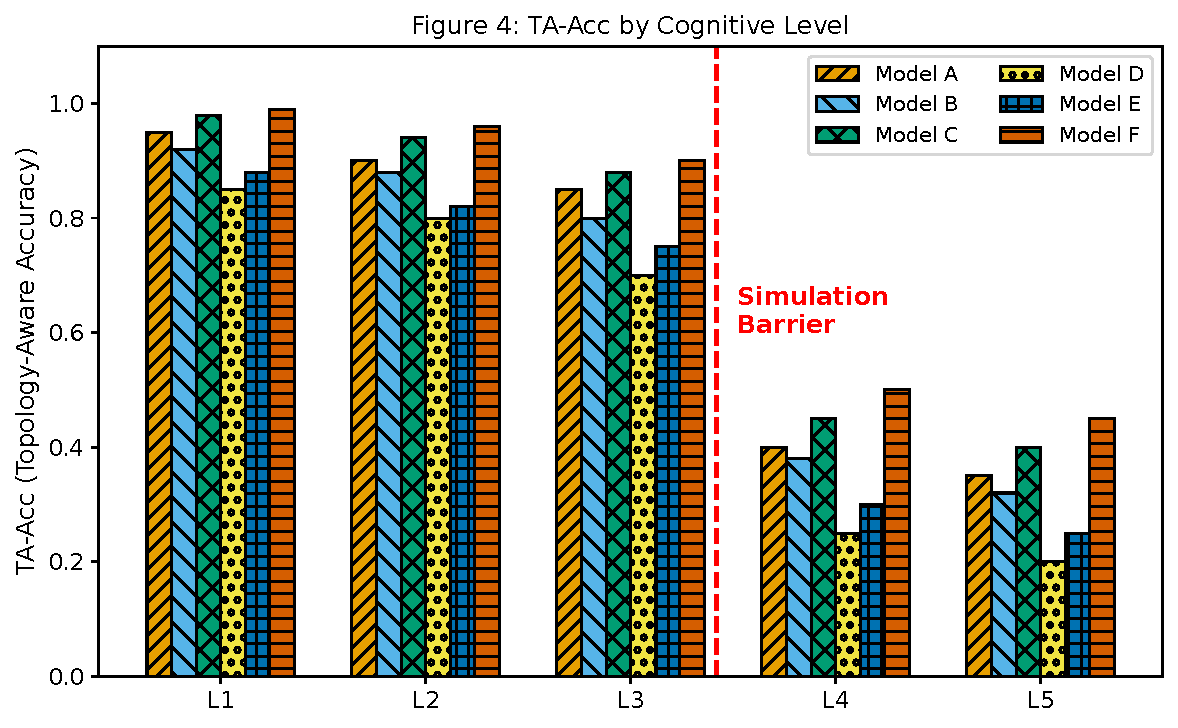
\includegraphics[width=\columnwidth]{fig4_ta_acc_levels}
  \caption{Lab-A에서의 인지 난이도별 TA-Acc. 이 그림은 6개 모델의 레벨별 성능 분포를 비교하기 위한 것으로, 점선은 본 연구가 시뮬레이션 장벽으로 해석하는 L3$\rightarrow$L4 경계를 나타낸다.}
  \label{fig:ta-acc-levels}
\end{figure}

\begin{figure}[!b]
  \centering
  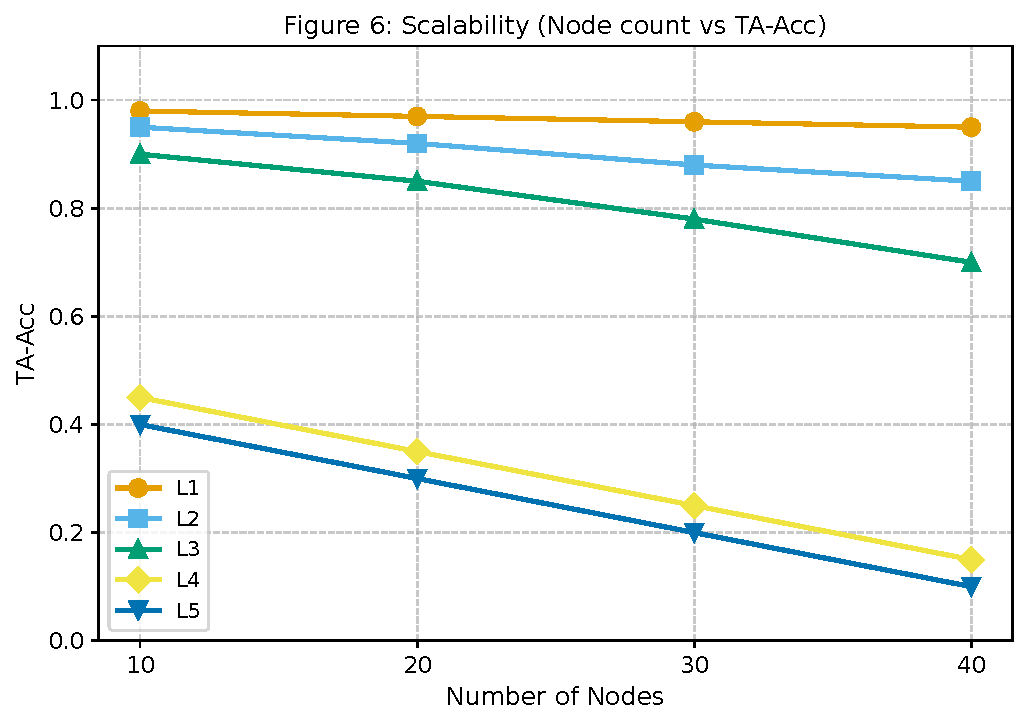
\includegraphics[width=\columnwidth]{fig6_scalability}
  \caption{토폴로지 규모에 따른 레벨별 TA-Acc 변화. 이 그림은 노드 수 증가에 따라 각 레벨의 성능이 어떻게 달라지는지 비교하기 위한 것이다.}
  \label{fig:scalability}
\end{figure}

\subsection{구조 효과와 도구 효과: 3-Way 비교}
도구 통합을 통한 시뮬레이션 장벽의 우회 가능성을 확인하기 위해, Section~V-B에서 Overall TA-Acc가 가장 높은 오픈소스 모델을 선정하여 세 가지 설정을 비교한다.
\begin{itemize}
  \item \textbf{Single LLM:} 도구 없음, 설정 파일 전문을 프롬프트에 포함 (Section~V-B 결과 재사용)
  \item \textbf{Pure MAS:} Orchestrator + Executor 구조, 모든 도구 비활성화. L4/L5 질문에 대해 Executor는 도구 호출 없이 프롬프트에 포함된 설정 파일만으로 경로 추론을 시도한다.
  \item \textbf{NetAlly:} Orchestrator + Executor + Batfish/NSO/PNETLab 도구 활성화
\end{itemize}
세 설정의 공정한 비교를 위해 다음 변인을 통제한다: (1)~동일 LLM backbone (Section~V-B에서 선정된 모델), (2)~동일 시스템 프롬프트 기본 구조 (Pure MAS와 NetAlly는 스킬 가이드 주입 여부만 상이), (3)~동일 최대 토큰 예산 및 최대 추론 단계 (max\_steps = 10), (4)~동일 설정 파일 입력. Pure MAS와 Single LLM의 차이는 질문 분해(Orchestrator의 스킬 선택)와 다단계 추론(Executor의 ReAct 루프)에 한정되며, 두 설정 모두 외부 도구에 접근할 수 없다. Pure MAS와 NetAlly의 차이는 도구 바인딩의 활성화 여부만이다. 따라서 $\Delta$(구조) = Pure MAS $-$ Single은 에이전트 구조(질문 분해 + 다단계 추론)의 효과를, $\Delta$(도구) = NetAlly $-$ Pure MAS는 동일 구조에서 도구 통합의 효과를 각각 분리한다. 다만, $\Delta$(구조)에는 질문 분해와 컨텍스트 재구성이 혼재하므로 순수 ablation이 아닌 준실험(quasi-experiment) 설계임을 유의한다.

\begin{figure}[!t]
  \centering
  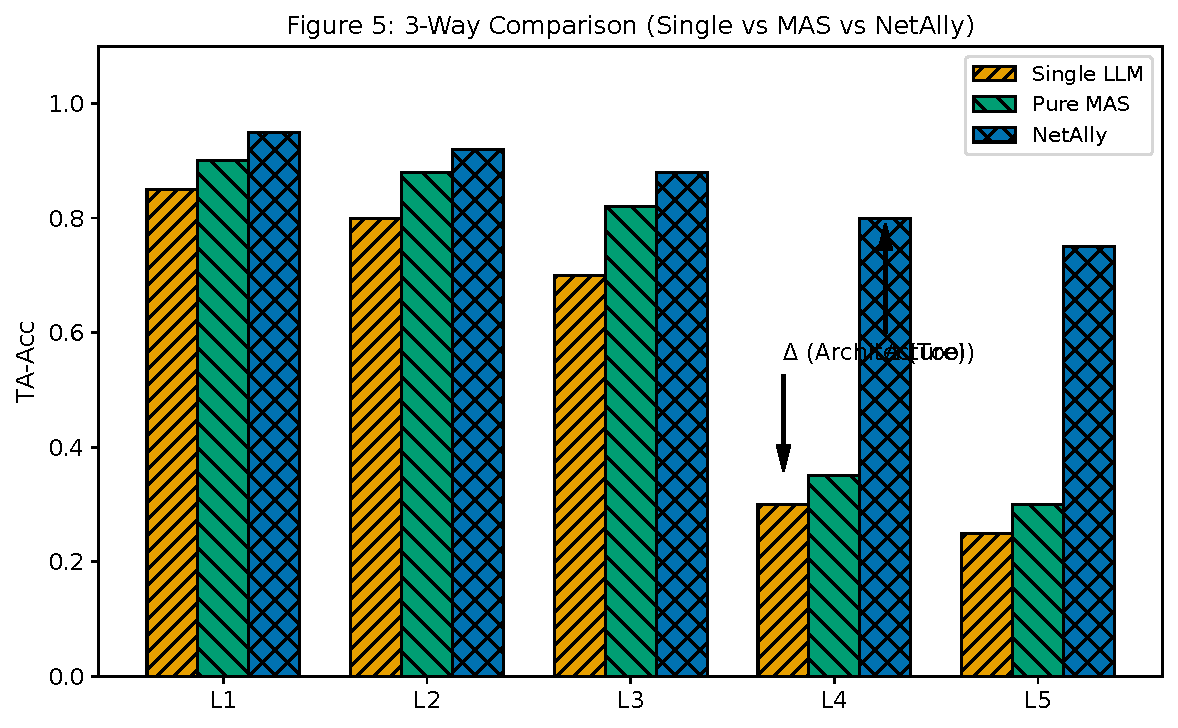
\includegraphics[width=\columnwidth]{fig5_3way_comparison}
  \caption{Single LLM, Pure MAS, NetAlly의 3-way 비교. $\Delta$(구조)는 Single$\rightarrow$Pure MAS, $\Delta$(도구)는 Pure MAS$\rightarrow$NetAlly의 차이를 나타내며, 구조 효과와 도구 효과를 분리해 해석하기 위한 도식이다.}
  \label{fig:three-way}
\end{figure}

\begin{table*}[!t]
  \caption{3-way 비교 결과}
  \label{tab:three-way}
  \centering
  \small
  \begin{tabular}{|C{1.2cm}|C{2.0cm}|C{2.0cm}|C{2.0cm}|C{2.0cm}|C{2.0cm}|}
    \hline
    \textbf{레벨} & \textbf{Single} & \textbf{Pure MAS} & \textbf{NetAlly} & \textbf{$\Delta$(구조)} & \textbf{$\Delta$(도구)} \\
    \hline
    L1          & TBD             & TBD               & TBD              &                       &                       \\
    \hline
    L2          & TBD             & TBD               & TBD              &                       &                       \\
    \hline
    L3          & TBD             & TBD               & TBD              &                       &                       \\
    \hline
    L4          & TBD             & TBD               & TBD              &                       &                       \\
    \hline
    L5          & TBD             & TBD               & TBD              &                       &                       \\
    \hline
  \end{tabular}
\end{table*}

\begin{table*}[!t]
  \caption{도구 호출 분석}
  \label{tab:tool-call-analysis}
  \centering
  \small
  \begin{tabular}{|C{1.2cm}|L{4.0cm}|C{2.0cm}|C{2.0cm}|C{2.0cm}|}
    \hline
    \textbf{레벨} & \textbf{주요 도구}         & \textbf{호출 성공률} & \textbf{TA-Acc (성공)} & \textbf{TA-Acc (실패)} \\
    \hline
    L4          & Batfish traceroute     & TBD             & TBD                  & TBD                  \\
    \hline
    L5          & Batfish fork\_snapshot & TBD             & TBD                  & TBD                  \\
    \hline
  \end{tabular}
\end{table*}

\subsection{오류 분석}
L4/L5 오답은 무작위 표본을 추출하여 오류 유형별로 분류한다(Table~\ref{tab:error-analysis}). 분석의 목적은 단순 정확도 비교를 넘어, 모델이 어떤 지점에서 추론을 중단하거나 잘못된 경로를 구성하는지 정성적으로 파악하는 데 있다. 특히 빈 응답 또는 추론 회피, 추가 홉 오류, IP-노드 매핑 실패, 형식 오류, 컨텍스트 포화는 L4/L5 성능 저하를 해석하는 핵심 후보 유형으로 간주한다. 최종 원고에서는 각 유형의 비율과 대표 사례를 함께 제시할 예정이다.

\begin{table*}[!t]
  \caption{L4/L5 오류 유형 분류}
  \label{tab:error-analysis}
  \centering
  \small
  \begin{tabular}{|L{2.8cm}|C{2.0cm}|L{7.0cm}|}
    \hline
    \textbf{오류 유형} & \textbf{비율} & \textbf{근본 원인}                    \\
    \hline
    빈 응답 / 추론 회피   & TBD         & 경로 계산 자체를 시도하지 못하거나 ``확인 불가''로 회피 \\
    \hline
    추가 홉 오류        & TBD         & 3홉 이상에서 중간 노드 누락 또는 불필요한 노드 추가    \\
    \hline
    IP-노드 매핑 실패    & TBD         & 목적지 IP의 소속 장비를 파악하지 못해 경로 과연장     \\
    \hline
    형식 오류          & TBD         & path/set 포매팅 실패로 파싱 불가            \\
    \hline
    Context 포화     & TBD         & 대규모 config 입력 시 답변 퇴화             \\
    \hline
  \end{tabular}
\end{table*}